\documentclass{main}
\begin{document}
\section{Invisible Internet Project - I2P}
This is a project trying to implement \textbf{Garlic Routing} - A Routing protocol built over onion routing.
It is not used widely as of today because it needs slightly more technical knowledge to set up for
the first time for use. Also, the sites outside the network of invisible internet cannot be accessed
through the invisible internet. One may access outside internet through proxies (which do exist) but 
the proxies may be malicious and it may not be safe to do so. This also is a big problem hindering the
popularity of i2p.

\subsection{I2P Protocol}
I2P adds more layers in Application Layer of primitive internet to introduce anonymity. Figure \ref{fig:i2p_protocol_stack}
shows the layers in this stack.

\begin{figure}[h]
	\centering
	\caption{I2P Protocol Stack}
	\label{fig:i2p_protocol_stack}
	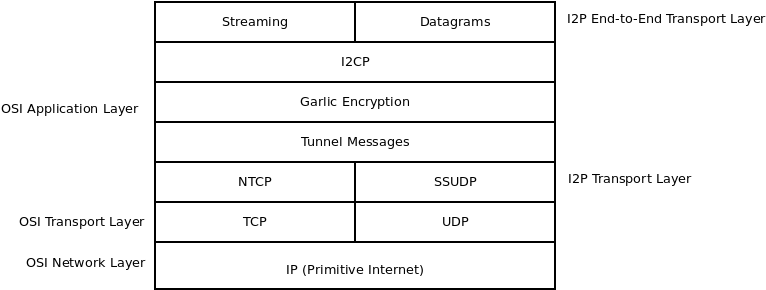
\includegraphics[width=\textwidth]{Resources/images/i2p_protocol_stack.png}
\end{figure}

I2P transport layer is built over Transport layer of regular internet. It is strictly for next-hop transfer
among I2P routers. This is non-anonymous transfer. This layer has two protocols built over TCP and UDP each.
\begin{itemize}
	\item NTCP2 - New I/O based TCP
	\item SSU - Secure and Semi-Reliable UDP
\end{itemize}

\subsection{Structure of I2P: Components}
\begin{itemize}
	\item \textbf{Tunnel} \\
		Messages are sent from one node to another through tunnels. There are two tunnels, outbound tunnel
		and inbound tunnel. This is needed as per Garlic Routing protocol. The sender first builds an 
		outbound tunnel. It gets the details of Inbound tunnel from netDB. \\
		In a tunnel a gateway refers to first router and the last router is called endpoint.
		A user might have multiple such outbound and inbound tunnels. These tunnels
		used in I2P are \textbf{unidirectional} as opposed to bi-directional routes in Tor. \\
		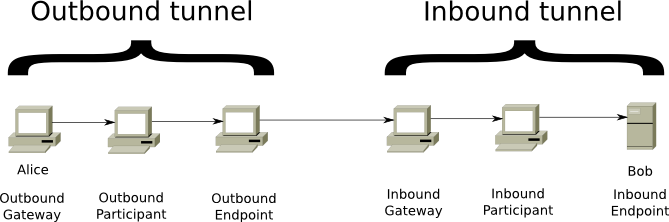
\includegraphics[width=0.95\textwidth]{Resources/images/i2p-tunnels.png}

		The sender adds routing instructions with the message, encrypts it and sends it through the tunnel.
		Just like Onion routing, this message is also encrypted using layered encryption. When the endpoint
		recieves the final message, it gets the routing instruction to the inbound gateway of reciever.
		The inbound gateway then sends this message to inbound endpoint through the tunnel. Except for this 
		difference, if we see tunnels as gateway to endpoint, both work in a similar way.

		Gateway accumulates some messages to be sent through the tunnel, adds path to reciever and
		converts them to \textbf{Garlic Message} so that they can be sent through tunnel.
		When the endpoint of tunnel finally decrypts the message, it separates the messages and forwards them 
		to the required hosts.
	\item \textbf{Network DataBase} \\
		Network Database stores the information about the routers present in the network. It also stores information
		about the tunnel gateways for inbound tunnels of users. In I2P, routers are identified by their public keys.
		This Network Database is a decentralized database. \\
		When a user wants to communicate with some other router in the Invisible Internet, he needs to lookup in the
		network database to find the details of inbound tunnel gateway for reciever. As it is a decentralized database,
		possibly, a router may not have access to complete database at any given time. As I2P is not widely used, it 
		is possible to find these details in a few tries but if the usage increases, it might become difficult to access
		this information.\\
		Network database stores two kinds of data: \textbf{leaseSets}(Section \ref{subsec:leaseSet}) and \textbf{routerInfo}(Section \ref{subsec:routerInfo})

\end{itemize}
\subsection{Network Database}
\subsubsection{Lease Sets}
\label{subsec:leaseSet}
Lease Sets are used to document tunnel entry points for a particular client destination. The following information is
stored in a Lease Set.
\begin{description}
	\item [Lease] stores information of the inbound tunnel gateway. A lease
		stores the following information. It is needed to send messages to the Destination.
		\begin{description}
			\item [Gateway Router] is specified for the tunnel. It is specified by spcifying it's identity.
			\item [Tunnel ID] to be used to send message through the tunnel.
			\item [Expiry Date] stores the time till when the tunnel is available.
		\end{description}
	\item [Destination] encryption key, signing key and a certificate.
	\item [Additional encryption public key] for use in encrypting garlic messages. It is used for end-to-end 
		ElGamal/AES + Session Tag encryption.
	\item [Signature] of the lease set to ensure that the data is published by the entity mentioned
		in destination.
\end{description}
There are various types of Lease sets like Unpublished Lease sets, Encrypted LeaseSets etc.

\subsubsection{Router Info}
\label{subsec:routerInfo}
RouterInfo includes the following details
\begin{description}
	\item [Router's Identity] stores an encryption key, a signing key and a certificate to authorize that.
		The public\_key is used for ElGamal Encryption in next-hop messages. The signing public key and
		key certificate are used for verifying signatures.
	\item [Contact Addresses] where the router can be reached. It contains mapping of transport protocol (NTCP or SSU)
		with ip address and port. 
	\item [Publish Date] is the time when this info was published.
	\item [Options] is a set of arbitrary options for telling the bandwidth capacities, router version, netId. There
		are some other stat options also.
	\item [Signature] of all the above data.
\end{description}
Router Info is stored in NetDB. This is required for building tunnels.
\end{document}
